\documentclass{thesis-ekf}
\usepackage[T1]{fontenc}
\usepackage[utf8]{inputenc}
\PassOptionsToPackage{defaults=hu-min}{magyar.ldf}
\usepackage[magyar]{babel}
\usepackage{graphicx,amsmath,amssymb,amsthm}
\graphicspath{{./images/}}
\footnotestyle{rule=fourth}

\newtheorem{tetel}{Tétel}[chapter]
\newtheorem{lemma}[tetel]{Lemma}
\theoremstyle{definition}
\newtheorem{definicio}[tetel]{Definíció}
\newtheorem{feladat}[tetel]{Feladat}
\theoremstyle{remark}
\newtheorem{megjegyzes}[tetel]{Megjegyzés}
\newtheorem*{megoldas}{Megoldás}

\logo{\includegraphics[width=8cm]{ekf-logo1}}
\institute{Eszterházy Károly Főiskola\\ Matematikai és Informatikai Intézet}
\title{Mobil eszköz alkalmazási lehetőségei fizikai kísérletekben}
\authorcaption{Készítette:}
\author{Asztalos Gergő\\ Programtervező informatikus}
\supervisorcaption{Témavezető:}
\supervisor{Biró Csaba\\ Adjunktus}
\city{Eger}
\date{2016}


\usepackage[T1]{fontenc}
\usepackage{inconsolata}
\usepackage{color}
\definecolor{bluekeywords}{rgb}{0.13,0.13,1}
\definecolor{greencomments}{rgb}{0,0.5,0}
\definecolor{redstrings}{rgb}{0.9,0,0}
\usepackage{listings}
\lstset{language=[Sharp]C,
	showspaces=false,
	showtabs=false,
	breaklines=true,
	showstringspaces=false,
	breakatwhitespace=true,
	escapeinside={(*@}{@*)},
	commentstyle=\color{greencomments},
	keywordstyle=\color{bluekeywords},
	stringstyle=\color{redstrings},
	basicstyle=\ttfamily
}


\begin{document}
\maketitle
\tableofcontents

\chapter*{Bevezetés}
A mai modern világban rohamléptekben nő az okostelefonok, táblagépek mindennapi felhasználása. Egyre több azon alkalmazások száma, melyek segítik, esetleg szórakoztatják vagy épp tájékoztatják a felhasználót egy adott témában. 
Szinte már mindenhez használjuk őket és kiaknázzuk az összes lehetőséget ahol újabb applikációval ismerkedhetünk meg.
Tanuláshoz, munkához is használjuk ezeket,bár nem lenne elengedhetetlen számunkra.
Sőt, annak ellenére, hogy az utolsó memóriát is lefoglaljuk ilyen programokkal az eszközeinkben, sok esetben meg sem fordul a fejünkben, hogy miből áll össze, milyen szoftveres vagy épp hardveres komponensek könnyítik meg az életünket. Én szerencsés vagyok, mert nem csupán eszembe jutott hanem választ is kaptam ezekre a "kérdésekre" az elmúlt három évben.
\par Amióta a főiskolára kerültem és programozni tanulok, egyre inkább foglalkoztatott, hogy hogyan is működik egy okostelefon, hogyan működnek a gesztusok, a tájolások, milyen eszköz segítségével tudja a telefon, hogy éppen hol vagyok. Miért képes egy relatíve kis eszköz megmutatni azt amit a hétköznapokban sokkal hatalmasabb eszközök szoktak mérni. Hogy képes több eseményt egy azon eszköz kezelni...
Később, tanulmányaim során megtudtam, hogy ezeket különböző szenzorok segítségével tudjuk elérni. 
Ezek a gondolatok megmozgatták a fantáziámat. Végül elkezdtem beleásni magam a témába: hogyan is lehetne ezeket még inkább beleszőni a mindennapjainkba. Hogy tudnánk használni ezeket a szenzorokat olyan célokra, melyek különböznek az átlagostól, esetleg még inkább segítik a munkánkat. Mi lenne, ha ezeket nem csak szórakozás, de tanítás céljából is fel tudnánk használni, elősegíteni a diákok fejlődését egy adott témakörben. Ezen célok eléréséhez a telefon egy jó segédeszköz lehet.
\par Ennek fényében szakdolgozatom témája a "Mobil eszköz alkalmazási lehetőségei, fizikai kísérletekben" lett, mert szeretném megmutatni, hogy az okostelefonokat lehet olyan célokra is használni, amelyekre az ember nem feltétlenül gondol azonnal. Hogy a gyerekek, ha már úgy is beviszik magukkal a tanórára a telefont, ne a közösségi életüket éljék rajta, hanem esetenként a tananyag elsajátítását is ennek az eszköznek a segítségével tegyék meg. Célkitűzésem tehát az lett, hogy készítsek egy olyan alkalmazást, mely segít a fizika tantárgy elsajátításában úgy, hogy egy segédeszközt ad a tanárok kezébe és egy olyan lehetőséget, mellyel megszeretteti a tantárgyat a diákokkal. Egy olyan alkalmazás, mely valós időben monitoroz különböző fizikai kísérleteket, felruházva azokat olyan adatokkal, amelyek szabad szemmel nem feltétlenül egyértelműek. Célom minél átláthatóbban, részletesebben felvázolni a program megvalósításának folyamatát és bemutatni a szakszerűen elkészített szoftvereket.
\chapter{Tervezés}
	Amikor egy projektről beszélünk, az első, és az egyik legfontosabb lépés az, hogy megfelelően megtervezzük a programunkat. Ezen folyamat során meg kell beszélnünk, hogy milyen lesz a program felépítése, struktúrája, designja. Fontos ezeket még a tervezési fázisban megtenni, hisz egy programnál bármit szeretnénk utólag módosítani, sokkal nehezebb lesz a feladatunk, mint az első lépésekben. Célszerű a tervezési fázisban megbeszélteket feljegyezni valamilyen formában. Ilyenkor sokan a rajzoláshoz, íráshoz folyamodnak és ezzel időt és energiát spórolnak maguknak.
	\par Én a tervezési szakaszt hasonlóan kezdtem el. Elsőként felépítettem a számomra megfelelő struktúrát, mindezt persze papíron, ceruzát használva. Tudtam, hogy nem csak egy alkalmazásom lesz, hiszen főbb céljaim között szerepelt a számítógép és okostelefon közötti Real-Time adatátviteli\footnote{Valós idejű adatfeldolgozás} kapcsolat kialakítása. Hasznos dolognak bizonyult még, a telefon szenzorainak kihasználása és azok alkalmazása a fizikában. Átgondoltam, hogy külön a telefonon és külön a számítógépen lévő programoknak milyen lenne a kinézete, milyen oldalak, ablakok követnék egymást. Elsőként az okostelefonra való fejlesztésnek láttam neki, azon belül is az Activity-k és Layout-ok kialakításába, mely a könnyebb része az egész programnak. Ezután el kellett gondolkoznom azon is, hogy miként fog kommunikálni az a két eszköz? Milyen szenzorral dolgozzak? Hogyan vigyem át az adatot úgy, hogy megközelítőleg valós idejű legyen?
	\par Természetesen az ilyen kérdésekre a válasz többnyire akkor derült ki, amikor már elkezdtem magát a programozást, megválaszolásukra pedig ismét csak papírt és tollat kellett ragadnom. A megfelelő adatokat, segédprogramokkal tudtam csak megjeleníteni, hisz az átlag felhasználók számára ezek a szenzoradatok lényegtelenek. Viszont ezekkel dolgozva, már tudtam készíteni diagramot, amellyel szemléltethettem, milyen értékekről is van szó és azokat hogyan tudnám alkalmazni az én projektemben.
\section{Accelerometer}
A gyorsulásmérő egy műszer, amely nevéből adódóan gyorsulás mérésére szolgál. A gyorsulást viszont elég nehéz mérni, ezért leginkább a gyorsuláskor fellépő erőt mérjük. Számtalan helyen használják és használhatják: okos telefonokban, digitális fényképezőgépekben, táblagépekben, repülésnél és még sok más helyen. Ezek a szenzorok alkotják a mikromechanikai szenzorok egyik nagy csoportját. A mérési elvek közül a legelterjedtebb a Newton 2. törvénye alapján működő elv, amelynek jellemzője a szeizmikus tömeg:
\begin{align*}
F=m\times a
\end{align*}
ahol a szenzor az $m$ tömegre ható $F$ erőt méri.
\subsection{Gyorsulásmérő okostelefonokban}
Okostelefonokban a gyorsulásmérő (Accelerometer) arra szolgál, hogy a készülék érzékelhesse a különböző mozgásokat, amikhez így feladatokat tudunk párosítani. A leggyakoribb és legelterjedtebb, az átlagos felhasználók által leginkább használt felhasználási módja az, amikor a telefont elforgatva a képernyő is automatikusan áttájolódik, fekvő és álló tájolási mód között váltakozva. Ez viszont (okostelefonokat tekintetbe véve) a legáltalánosabb felhasználási módszer, ezen kívül még számos esetben használhatjuk a gyorsulásmérőnket, így például gesztusok kezelésében\footnote{A telefont megrázva valamilyen irányítást eszközlünk}, de akár játékok irányításában is.
\subsection{Gyorsulásmérő alkalmazása a fizikában}
Ahogy a példák is mutatják, számos dologra használhatjuk szenzorunkat, miért ne használnánk tehát fizikai kísérletekben segédeszközként? Amikor ilyen kísérletekről beszélünk, természetesen nem olyan kísérletekre gondolunk, ahol a telefon víz vagy tűzállóságát teszteljük, esetleg a szabadesést vizsgáljuk, viszont egy inga használatára kiváltképp alkalmas lehet. Kihasználva a telefonra ható gravitációs erőt, illetve a gyorsulást, máris monitorozni tudjuk a telefonunkat, és használhatjuk segédeszközként.
\section{A felület}
Mint mindenkinek, nekem is elsők között szerepelt a tervezési szakaszban a felület megtervezése. Ehhez nem használtam külső szoftvert, inkább papírformán készítettem el a drótvázat. Miután már tudtam, milyen funkciói lesznek a programomnak, itt volt az ideje, hogy megtervezzem a felületét. Számomra nem az volt a legfontosabb, hogy működő, jól áttekinthető legyen, a kinézet csak másodlagos volt. Mivel több megjelenítési forma, vagy adott esetben kísérlet is lesz, szükség volt valamilyen módszerre. Ehhez RadioButton-öket választottam. Ez azért tűnt optimálisnak, mert mindig csak 1 gomb lehet bekapcsolva, így váltani lehet a kísérletek között. Ezen kívül szükség volt még arra, hogy a szenzor értékeit kiírassam, ehhez pedig Label-t használtam. A gyorsulási grafikon megjelenítéséhez egy beépített eszközt találtam alkalmasnak, ami nem más, mint a Chart. Ez egy olyan eszköz, amelynek segítségével diagramokat rajzoltathatunk ki, pusztán úgy, hogy pontokat adunk hozzá.
Ezek mellett természetesen szükség volt egy kapcsolódás gombra is, hiszen valahogy kapcsolatot szeretnénk létesíteni a telefonunkkal.
\par Az Android applikáció felületét hasonló módon terveztem meg, habár az sokkal szolidabb, kevesebb Tool helyezkedik el rajta. Itt 2 Activity-t terveztem meg. Az első lényegében csak 2 TextBoxot és egy Connect gombot tartalmaz, melyek segítségével létrehozhatjuk a kapcsolatot. A második Activity esetében hasonló a dolgunk, hisz ott is csak egy pár eszköz lesz a képernyőn. Pár darab Label, RadioButton, hasonlóan a szerver oldali applikációhoz, azért, hogy a szenzor mérési gyorsaságát be lehessen állítani. Továbbá kell még egy Switch gomb is, hogy a felhasználó váltani tudjon a filterezett szenzor mérés és a tiszta mérés között. 
\chapter{Szerver alkalmazás}
Miután megterveztem, milyen is lesz a programom, kialakítottam egy drótváz modellt, és fejben már tudtam, hogyan fog működni az applikációm, itt volt az ideje, hogy elkészítsem a szerveroldali alkalmazásomat is.
\par Első, és talán az egyik legfontosabb feladatom az volt, hogy eldöntsem, milyen nyelven fogom elkészíteni. Több nyelv is bekerült a számomra aktuális nyelvek listájába. Felmerült az is, hogy Python lesz a választott nyelv, hiszen a hasonló matematikai vagy fizikai megoldások felettébb optimalizáltak és a futási ideje sem másodlagos.
\par A választásom mégis csak a C\# nyelvre esett, ennek pedig nem egy oka van. Talán azért is választottam ezt a nyelvet, mert tudtam, hogy az internet adta segítségeket leszámítva is el tudom készíteni az alkalmazásom, hiszen már a főiskolán is ez volt az első nyelv amivel megismerkedtem és nagyon sok segítséget kaptam az oktatóimtól is. Külön tantárgy foglalkozott a grafikai rajzolással, megjelenítéssel, s mivel a témámhoz szükségem volt ezekre, megerősített abban, hogy ennél a nyelvnél maradjak. Továbbá a fejlesztői környezet ismerete is megkönnyítette a munkámat, hisz nem kellett újjal megismerkednem. Ez a fejlesztői környezet pedig a Visual Studio volt.
\section{Visual Studio}
A Visual Studio a Microsoft olyan fejlesztői környezete, mely több nyelvet is tartalmaz mint plédául a Visual Basic, C++, C\# és ezek mellett még a z XML-t\footnote{Extensible Markup Language - Kiterjeszthető jelölő nyelv} is támogatja, ezek a nyelvek pedig mind IDE\footnote{Integrated Development Environment, azaz integrált fejlesztői környezet} fejlesztői környezetet használnak. Különböző Project Template-k közül választhatunk, mint például a Console Application, Windows Form Application, Windows Presentation Foundation. A Visual Studio egy meglehetősen jó fejlesztői környezet, melynek egyszerű és áttekinthető a fájl struktúrája, így könnyebbé és gyorsabbá teszi a munkát a felhasználója számára. A Project Template-ket böngészve sokat tűnődtem azon, hogy melyiket is válasszam, de végül a Windows Form Application-nél maradtam. 
\par Ezt azért választottam, mert a tervezési folyamatnál már tudtam, hogy létre kell hoznom egy TCP/IP kapcsolatot a telefon és a számítógép között, emellett azt is, hogy valamilyen formában rajzolni szeretnék a formomra, habár azt, hogy pontosan mit, abban még nem voltam biztos.E témában és ebben a környezetben már voltak korábbi tapasztalataim, éreztem, hogy képes leszek megvalósítani.
\section{TCP/IP kapcsolat}
A Transmission Control Protocol, azaz TCP, az internet egyik legfőbb részét, az úgymond "gerincét" alkotó TCP/IP protokollcsalád egyik fő protokollja. Ezen protokollcsalád két legfontosabb transzport protokollja a TCP és az UDP\footnote{User Datagram Protocol}. A TCP egy kapcsolatorientált, megbízható protokoll. A kommunikáció megkezdése előtt ki kell építenünk a kapcsolatot, majd ezután megkezdhetjük az adatátvitelt. Amennyiben hiba történik, mint például elveszik egy csomag, vagy meghibásodik, esetleg már hibásan érkezik, a TCP saját maga újraindítást kér. Az átvitel úgy történik, hogy az adat, amit szeretnénk átküldeni egy úgynevezett byte-folyam, amit a TCP szétszeparál csomagokra és elküldi. A kapcsolat tehát full-duplex\footnote{Megengedi a kétirányú kapcsolatot, szimultán módon}, továbbá rendelkezik egy olyan szinkronizációs mechanizmussal, ami megakadályozza, hogy az adó elárassza a vevőt. Emellett a TCP figyeli a kapcsolatot és megpróbálja megtippelni a sávszélességét a torlódásokból, válaszidőből stb., amit később felhasznál az adatsebesség beállításakor.
\par Az én programomat nézve az okostelefon minősül az adónak és a számítógép a vevőnek. Értelemszerű, hiszen a szenzoradat a telefonról érkezik és azt kell továbbítanunk a vevőnek. Ez úgy történik, hogy a telefon egy IP cím és egy Port szám segítségével kérést küld a szerveroldal felé a kapcsolódásra, amit a már várakozó szerver később fogad. Ezután meg is kezdődik az adatátvitel. Esetünkben, mivel az egész program a RealTime adatátvitelen alapszik, ezért a kommunikáció nyitott, mindaddig, míg azt "erőszakkal" be nem zárjuk.
\subsection{Adatok feldolgozása}
Az élő kapcsolat fenntartása annyit jelent, hogy a beérkező adatot azonnal feldolgozzuk és a célunknak megfelelően fel is használjuk, adatról-adatra. A hangsúly azon van, hogy megpróbáljuk abban a pillanatban feldolgozni szerver oldalon az adatot, amikor az előállítódik a kliens oldalon. Természetesen száz százalékosan ez nem teljesíthető, hiszen ez a folyamat elég erőforrás igényes.
\par A kapcsolat beérkezése után meg is kezdődik az adatok feldolgozása. Ez a feldolgozási folyamat természetesen attól függ, mit szeretnénk csinálni az adatunkkal.
\begin{lstlisting}
int port = 8888;
label5.Invoke(new Action(() => label5.Text = GetLocalIPAddress()));
TcpListener myListener = new TcpListener(IPAddress.Parse(GetLocalIPAddress()), port);
myListener.Start();
label1.Invoke(new Action(() => label1.Text = "Varakozas kliensekre a " + port + " porton."));
TcpClient connectedClient = myListener.AcceptTcpClient();
label1.Invoke(new Action(() => label1.Text = "Kliens csatlakozott"));
\end{lstlisting}
A csatlakozást követően szükségünk van egy StreamReader-re, ahhoz, hogy a kapcsolódott eszköz által küldött információt meg is tudjuk jeleníteni, vizsgálni.
Az adatok, azaz a 3 tengely értéke 1 adott sorként érkezik át a kapcsolat folyamán. Ha ezekkel az adatokkal dolgozni is szeretnénk (márpedig szeretnénk), szükségünk lesz arra, hogy azt az 1 sort, szétbontsuk 3, különálló értékre. Így megkapjuk az x, y és z tengelyek értékét.
\begin{align*}
-0,10534488 \qquad 9,787497 \qquad-1,091756
\end{align*}
 A szétbontásuk pedig a következőképp történik:
 \begin{lstlisting}
 string s = r.ReadLine();
 string[] str_array = s.Split(' ');
 x = double.Parse(str_array[0], CultureInfo.InvariantCulture);
 y = double.Parse(str_array[1], CultureInfo.InvariantCulture);
 z = double.Parse(str_array[2], CultureInfo.InvariantCulture);
 \end{lstlisting}
Ebben az esetben a(z) $s$ változónk tárolja az átküldött sort, a(z) $str_array$ pedig annak a szétbontott változatát. Így meg is kaptuk a szövegként átküldött sorunkat, változókra szétbontva és megkezdhetjük a feldolgozásukat, beillesztésüket a feladatunkba.

\section{Kísérletek}
\subsection{Gyorsulás diagram}
Most már megvannak az adataink, fel is tudjuk hát dolgozni őket. Első és legfontosabb dolgunk az, hogy létrehozzunk egy diagramot, ami segítségével meg tudjuk jeleníteni (tengelyenként) a telefonunk gyorsulását. Ez már önmagában véve is egy olyan szemléltetés, melyet használhatnánk a fizika tanórákon. Szerencsére van erre egy beépített Tool\footnote{Visual Studio-ban a felhelyezhető gombokat, mezőket egy ToolBoxban találjuk}, melynek értékeket átadva már el is készíti a megfelelő diagramot. Ezen Tool neve: Chart. Dolgunk nehezedik annyiban, hogy ennek a diagramnak előre definiálnunk kell bizonyos pontokat a megjelenítéshez, viszont bármikor tudunk hozzáadni új pontokat. Ezzel csak annyi a probléma, hogy az új pontokat beszúrja, a többi pont mellé, így viszont bizonyos idő után feltorlódnak az adatok és a vonaldiagramunk elveszti varázsát. 
\begin{figure}[!h]
	\centering
	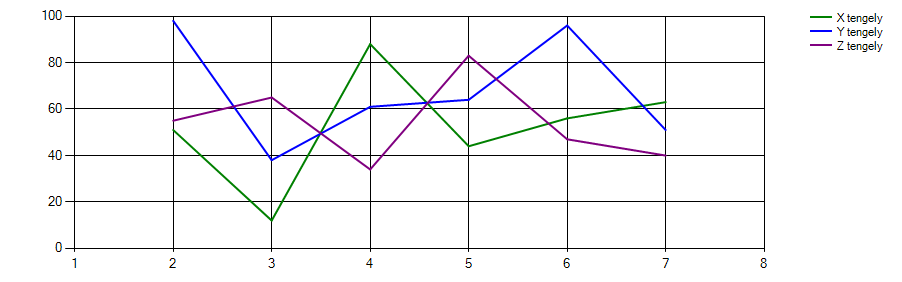
\includegraphics[width=15cm]{grafikon}
	\caption{Gyorsulás grafikon}\label{grafikon}
\end{figure}
\par Erre beépített megoldásunk sajnos nincs, magunknak kell megírnunk a függvényünket úgy, hogy a bent lévő adatok egy része megmaradjon, viszont a régi adatokat kitöröljük. Erre egy olyan megoldást eszközöltem, hogy amennyiben a diagramunk pontjainak száma elér egy előre megadott mennyiséget, a pontokat elmentjük egy listába, a listát megfelezzük, az első részét töröljük a diagram összes elemével együtt, majd a lista második része lesz a diagramunkra ráillesztve. Ezzel azt érjük el, hogy a diagram törlődik, az elemek fele elvész, a másik fele pedig újból beíródik, így a diagramunknál nem lesz torlódás, mégis folyamatosnak látszik a megjelenítés.
\subsection{Inga}
Sokszor elgondolkoztam azon, hogy ha már ennyi mindenre képesek a telefonjaink a mai világban, miért ne használnánk őket a Chatelésen és a fénykép készítésen kívül valami másra is, valami hasznosabbra esetleg. Természetesen a telefon legfőbb célja még mindig a telefonálás, de mi lenne, ha például egy inga lemodellezésére tudnánk használni, esetleg fizikai tanórákon?
\par Számtalan internetes fórumot és hasonló oldalt átnéztem, de sehol nem találtam olyan megoldást, amelyben a telefon valamelyik szenzorát úgy használják ki, hogy az valós időben monitorozva legyen esetleg egy számítógépen is, kirajzolva azon az egyes fizikai adatait az ingamozgásnak, vagy ha esetleg volt is, nem valós idejű. Elkezdtem gondolkodni, hogyan is lehetne megoldani, ezt a fajta monitorozást. Az első dolog ami eszembe jutott, hogy megvizsgáljam, milyen adatokat kapunk, egy-egy mérés során? Nos, igaz hogy a gyorsulásmérőt nem feltétlenül erre találták ki, de az adatok olyan biztatóak voltak, hogy nyugodtan lehetett velük tervezni. Ezután már csak az jött, hogy hogyan használjam fel ezeket az adatokat?
\begin{figure}[!h]
	\centering
	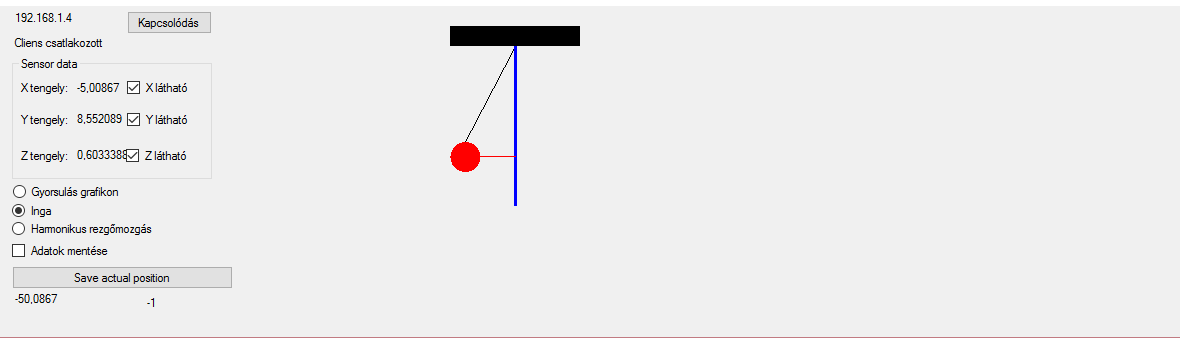
\includegraphics[width=15cm]{inga}
	\caption{Inga}\label{inga}
\end{figure}
\par A megoldás az lett, hogy figyelembe véve az ablak méretét (magasság/szélesség), amire rajzolni szeretnénk (tehát megjeleníteni az ingánkat) és az adatokat összevetve, arra jutottam, hogy a telefon mért tengelyadatait, a képernyőre vetítve akár még megfelelő megoldást is kaphatok. A szenzoradatok viszont nem egész értékek, hanem valós számok, szemben a képernyő szélesség vagy magasságával, hiszen azok pixelszámok, amik minden esetben egészek. Át kellett tehát konvertálni a szenzoradatunkat egész számmá, kerekítve azt. Ennek eredménye pedig az lett, hogy a telefon inga-mozgása már lekövethető lett a képernyőn is. 
 \begin{lstlisting}
float xPoint = Convert.ToSingle(Nx) + 500;
float yPoint = Convert.ToSingle(Ny) + 50;
//"Fonal"
g.DrawLine(pendPen, 515, 40, xPoint+15, yPoint);
//Thetajelzo vonal
g.DrawLine(new Pen(Color.Red),515,150,(float)Nx+515,(float)Ny+65);
//A telefont helyettesito test
g.FillEllipse(new SolidBrush(Color.Red), ((float)Nx+500), ((float)Ny + 50) , 30, 30);
 \end{lstlisting}
 \par Tehát lényegében annyi történik, hogy minden egyes szenzoradat mérésnél behelyettesítjük a telefon új pozícióját a rajzoló függvényünkbe. Ennek hatására egy folyamatosnak tűnő mozgást érünk el. Ha rezgőmozgásról beszélünk, két fajta rezgőmozgást különböztetünk meg:
\subsection{Harmonikus rezgőmozgás}
A harmonikus rezgőmozgásról akkor beszélünk, ha egy testet az egyensúlyi helyzetéből kimozdítunk, és ennek köszönhetően a test két szélső helyzet között periodikus mozgást végez.
\begin{enumerate}
	\item Csillapítatlan rezgőmozgás: Időben állandó a maximális kitérés (idealizált eset).
	\item Csillapított rezgőmozgás: A maximális kitérés időben csökken.
\end{enumerate}
\par Ha egy kicsit jobban bele szeretnénk mélyülni a fizikába, megvizsgálhatjuk az idő szinuszos függvényét is. Ebben az esetben, ha egy rugóra függesztett test rezgését vizsgáljuk, és azonos időközönként megfigyeljük a kitérést, akkor azt tapasztaljuk, hogy a kitérés az idő szinuszos függvénye lesz.
\begin{figure}[!h]
	\centering
	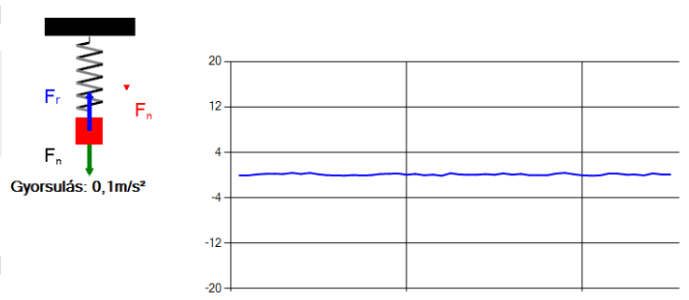
\includegraphics[width=15cm]{harmonikus}
	\caption{Harmonikus rezgőmozgás}\label{harmonikus}
\end{figure}
\par A tervezési szakaszban, az ingán gondolkodva, eszembe juttatott még egy kísérletet, ami hasonló elven működik és szemléltetésnek se a legrosszabb dolog, ez pedig a Harmonikus Rezgőmozgás. A gyorsuló mozgást minden irányból, minden tengelyen tudjuk mérni. Rezgő mozgásnál azonban csak egy adott tengelyre van szükségünk, mégpedig az Y tengelyre. Ennél a kísérletnél biztos hogy mindig ezt a tengelyt fogjuk figyelni, hiszen biztos, hogy a telefon állított pozícióban lesz és az is biztos, hogy mi csak a le-fel mozgását fogjuk figyelembe venni.  Tehát az olyan rezgőmozgást, ahol teljesül, hogy a kitérés az idő szinuszos függvénye harmonikus rezgőmozgásnak nevezzük.
 \begin{lstlisting}
g.DrawLine(515,40,515,Convert.ToSingle(Ny)+100);
 \end{lstlisting}
\par A rajzolás pozicionálásához természetesen szükségünk van olyan konstans értékekre, amik csak azt adják meg, hogy nagyjából hova rajzoljunk, hiszen ha csak a szenzoradatra támaszkodnánk, akkor nem feltétlenül azzal az eredménnyel szembesülnénk, amire vártunk.
\par Szükségesnek találtam még azt is, hogy feltüntessem a kísérlethez megfelelő vektorokat. Esetünkben, ha egy kísérlet szemléltetéséről van szó, akkor a lehető legtöbb információt megjelenítjük, segítve ezzel a felhasználót, hogy jobban megértse miről is van szó az adott ábrán. A mozgásnál fellépő, illetve az testre ható erők szemléltetése épp olyan fontos, mint maga az inka kirajzolása.
\par Mellékeltem továbbá a rezgőmozgás ábrája mellé az egy tengelyre ható gyorsulás grafikont is, hisz mozgás közben ennek is fontos szerepe van, ha szemléltetésről beszélünk. Azonnal érthetőbb lesz a kísérletünk, bármely felhasználó számára, kisebb kiegészítésekkel.
\subsection{Egyéb alkalmazható kísérletek}
Az egész keretrendszer felépítése lehetővé teszi azt, hogy kisebb programkód átírással bármilyen fizikai kísérletet megvalósítsunk, amennyiben azt lehetséges. Számtalan kísérlet van még, amit megvalósíthatunk, letesztelhetünk, habár megjelenítésük nem a legegyszerűbb. A cél az, hogy a fizikát, mint tantárgyat vagy mint szakterületet még jobban meg lehessen szerettetni a diákokkal, esetleg érdekesebb legyen egy-egy óra tartalma. A mai modern világban a hasonló megközelítésű, beállítottságú ötletek mindenkinek, de leginkább a fiatalabb korosztálynak biztosan felkeltik a figyelmét.
\par Ilyen lehet például, mikor kamera segítségével szeretnénk lemérni egy tárgy sebességét. Ilyen, vagy ehhez hasonló alkalmazást már készítettek is, melynek lényege, hogy a tárgyra irányítva a kamerát, megtudhatjuk annak sebességét.
\subsection{Kísérletek grafikus megjelenítése}
Amikor egy adott témában, megjelenítésről beszélünk, mindenkinek máshogyan fogalmazódik meg a fejében, hogy miről is van szó. Az én programomnál azt akartam, hogy minél jobban, minél élethűbben vissza tudjam adni azt, ami a valóságban történik. Adott esetben, például ha egy ingáról van szó, ugyanúgy egy ingát szeretnénk látni, mint ahogy a valóságban is. Éppen ezért én a $C\sharp$ Graphics osztályát használtam ahhoz, hogy ki tudjam rajzoltatni az adott testet. Ehhez szükség van arra, hogy bepozicionáljuk a testet, adott esetben az ingát, úgy, hogy figyelembe vesszük annak mozgását. Ezt úgy valósulhat meg, ha kirajzoltatunk 2 testet, az egyik a fonál a másik pedig a fonál végére "kötött" test, melyeknek olyan koordinátát adunk, ami segítségével elérhetjük a folytonos mozgást. Ha a form felületére rajzolunk valamit, muszáj minden egyes kirajzoltatás előtt letörölni azt, ellenkező esetben azt fogjuk látni, hogy tele lesz rajzolva az adott ablakunk, és nem olyan lesz az eredményünk mint amire vártunk. Ehhez az Invalidate() és Update() beépített függvényeket hívjuk meg. Hatásukra minden kirajzoltatásnál törlődik a képernyő, mielőtt újra rajzolnánk rá.
\begin{lstlisting}
Invoke(new Action(() => Invalidate()));
Invoke(new Action(() => Update()));
Graphics g = CreateGraphics();
//Fonal
g.DrawLine(new Pen(Color.Blue, 2),515,40,515,Convert.ToSingle(Ny)+100);
//Telefon helyettesito test, esetunkben egy kitoltott kor
g.FillEllipse(new SolidBrush(Color.Red), 500, Convert.ToSingle(Ny) + 100, 30, 30);
\end{lstlisting}
\chapter{Kliens alkalmazás}
Mivel a szenzoradatok feldolgozását esetemben fizikai kísérletek végrehajtásához használnám fel, figyelembe kellett vennem, hogy ne legyen túlságosan hardverigényes a programom. Ezért is választottam a gyorsulásmérőt, mint szenzort, mivel az manapság szinte minden Androidos eszközben megtalálható, így nem kell abba időt, pénzt és energiát fektetnünk, hogy megfelelő eszközt találjunk, szinte minden eszköz megfelel számunkra. Az okostelefon tájolását tekintve nem kell nagy figyelmet fordítanom arra, hogy milyen irányban is van a telefon, ()amennyiben a programról beszélünk). Ellenben fontos,hogy hogy milyen kísérletet szeretnénk ábrázolni, megjeleníteni. Mégpedig azért fontos, mert a tengelyek, amiket használunk fix pozíción vannak, viszont ha telefont elfordítjuk, akkor a megfigyelt tengelyünk horizontális/vertikális állásból ellenkező állásba kerül. Így az adatok is máshogyan fognak megjelenítődni.
\par A tervezésnél kialakítottam 2 Activity-t\footnote{Activity, más néven Form, azaz eg yoldalt jelent.}, az egyik a kapcsolódásra szolgál, a másik pedig a szenzoradatokat jeleníti meg, továbbá lehetőséget ad a szenzor mérési gyorsaságának beállítására és a filterezés beállítására. Igaz, a megjelenített oldalunkon nem lesz sok adat feltüntetve, de a háttérmunka, a számítások, pontosítások amiket a telefon végez, fontosabbak, mint az, hogy kinézetre milyen az alkalmazásunk.
\begin{center}
	\begin{tabular}{ |c|c|c| } 
		\hline
		Tengely: & Szenzor adat \\
		\hline\hline
		X: & -0,10534488  \\
		\hline
		Y: & 9,787497 \\
		\hline
		Z: & -1,091756 \\
		\hline
	\end{tabular}
\end{center}
\par Szükségünk lesz továbbá arra, hogy a mért szenzoradatokat némely esetben pontosítsuk, filterezzük. Erre csak pár kísérletnél van szükség, viszont ez éppen elég indok ahhoz, hogy lehetőséget biztosítsunk a felhasználónak a választásra a tiszta szenzoradatok és a pontosítottak között.
\par Természetesen nem csak ezt az egy szenzort lehet kihasználni ilyen kísérletek végrehajtásához, szemléltetéséhez. Jó pár szenzor van még a telefonban mint például a Gyroscope, vagy akár a mikrofon, de még a kamerát is kihasználhatjuk valamilyen kísérlet bemutatásához, akár szabadesést szeretnénk szimulálni, vagy a hang terjedését kívánjuk szemléltetni.
\par Az okostelefon szenzorokat is két külön csoportra bonthatjuk. Hardveres szenzor illetve Szoftveres szenzor. Ezek nevükből adódóan olyan szenzorok, melyek vagy be vannak építve a telefonba, vagy egy másik szenzort és egy kis szoftveres ügyeskedést felhasználva, szimuláljuk azt.
\begin{center}
	\begin{tabular}{ |c|c|c| } 
		\hline
		Szenzor: & Típus: \\
		\hline\hline
		Accelerometer / gyorsulásmérő & Hardver  \\
		\hline
		Környezeti hőmérséklet szenzor & Hardver \\
		\hline
		Gravitációs szenzor & Szoftver vagy Hardver \\
		\hline
		Gyroscope & Hardver \\
		\hline
		Fény szenzor & Hardver \\
		\hline
		Orientation / Tájolás & Szoftver \\
		\hline
	\end{tabular}
\end{center}
\section{Android Studio}
A szerver oldalt követően a mobil alkalmazás fejlesztését is el kellett kezdenem. Ehhez én az Android Studio-t\footnote{Fejlesztői eszköz amit a Google adott ki} választottam. Itt alakítottam ki a kapcsolódáshoz szükséges képernyőt, a szenzoradat megjelenítő képernyőt és a fontosabb részeket. De még mielőtt belefolynánk ezen fejlesztői környezet szerepét, tisztáznunk kell pár lényegesebb dolgot, ami nem feltétlenül egyértelmű mindenki számára.
\par Mi az hogy Android? Az Android napjaink egyik legsikeresebb mobil  operációsrendszere. Bizonyos statisztikák szerint több száz millió Android-alapú készülék van már a piacon és ez a szám egyre csak nő és nő. Naponta több száz-ezer készüléket aktiválnak. A rendszernek régen külön verziója létezett telefonkészülékekre és táblagépekre, ám 2012-ben megjelent a 4.0-s verzió, amely már egyesíti ezt a két külön ágazó útvonalat, így manapság már minden eszközön egyazon verzió fut.
\par A platform népszerűségét nagyon sok tényezőnek köszönheti, melyek közt szerepel a kiemelkedően látványos felhasználói felület, a könnyű használhatóság, a nyíltság és a magas fokú kompatibilitás. Ám nem csak ezeknek köszönheti népszerűségét. Fontos szerepe van az operációs rendszert futtató készülékek hardverképességeinek, a gyors processzornak és a nagy méretű memóriának.
\par Az androidon egyrészt magát a mobil operációsrendszert értjük, másrészt pedig a futtató eszközt. A Google 2005-ben felvásárolta az Android Incorporated nevű vállalatot és ezután saját maga kezdte el a fejlesztést, így részben az Android a Google fejlesztése.
\par Az Android fejlesztését tekintve eléggé barátságos, ugyanis ingyenes és nyílt forráskódú az operációsrendszer. Hivatalosan az Open Handset Alliance konzorcium fejleszti és a Google a vezetője.
\par Számos fejlesztői környezet adódik, az ismeretlenektől kezdve az ismertekig, ám én mégis az Android Studio-t választottam. Ennek legfőbb oka az lehet, hogy a barátságos megjelenését, emberbarát fájl struktúráját és azt a tényt, hogy már fejlesztettem benne, tartottam szem előtt.
\begin{center}
	\begin{tabular}{ |c|c|c| } 
		\hline
		Fejlesztői környezet & Előnye & Hátránya \\
		\hline\hline
		Android Studio & Ingyenes, nyílt forráskódok & Lassú buildelés\footnote{A kész programot futtatjuk az eszközön}  \\
		\hline
		Eclipse & "helyetted írja a kódot" & Nagy memória felhasználás\\
		\hline
		Visual Studio & Erőforrás mérés & Nem Androidra fejlesztették \\
		\hline
	\end{tabular}
\end{center}
\section{Az alkalmazás}
Mint már említettem, a kliens alkalmazásom csak 2 képernyőt tartalmaz. Az elsődleges a kapcsolódáshoz szükséges adatokat kéri be (IP cím, Port), a második pedig a szenzor feldolgozást hajtja végre. Ez előbbi úgy történik, hogy felcsatlakozunk a WiFi-re a szerver alkalmazással, majd az általa kapott IP-címre rácsatlakozunk a kliens alkalmazással. Triviális tehát hogy elsőként a szerver alkalmazásnak kell futnia, csak utána tudunk csatlakozni a klienssel. Tehát miután beírtuk a megfelelő címet, melyre kapcsolódni szeretnénk, az alkalmazásunk továbbmegy a következő ablakra. A tényleges kapcsolódás itt történik, az előzőnél még csak elkértük a címet. Ez a lépés azért fontos, mert így a felhasználó anélkül is használhatja az alkalmazást, hogy lenne internet elérése. Ilyenkor az alkalmazás csak egy üzenetet küld, miszerint nem éri el a szerver oldalt, funkcióiban pedig közel ugyanazt nyújtja.
\subsection{AsyncTask}
Az AsyncTask egy olyan metódus, mely segítségével a háttérben futó időigényes feladatokat tudjuk megoldani. Ezt a programunk fő szálától elkülönítve tudjuk megtenni a segítségével, ugyanis a fő szálat (User Interface) nem állíthatjuk le hosszú időre, ilyenkor ugyanis semmiféle felhasználói utasításra nem reagál. Éppen ezért, ezeket a feladatokat a háttérben, egy background szálon kell futtatnunk. Tehát lényegében a felhasználói szál és a háttérben dolgozó szál egyszerre fut. Természetesen előfordul, hogy ezek időnként kommunikálnak. 
\par Éppen ezért, a kapcsolat kezelését én egy AsyncTask metódus segítségével oldottam meg. Kicsit nehezítette a feladatot az is, hogy miközben a kapcsolat él, megállás nélkül kommunikálunk a szerverrel, így aztán a felhasználói felületnek néha bele-bele kell nyúlnia a másik szálba.
\begin{lstlisting}
protected Void doInBackground(Void... arg0) {
try {
    socket = new Socket(ipAddress,portN);
    ByteArrayOutputStream byteArrayOutputStream =
    new ByteArrayOutputStream(1024);
    byte[] buffer = new byte[1024];
    int bytesRead;
    InputStream inputStream = socket.getInputStream();
    while ((bytesRead = inputStream.read(buffer)) != -1){
        byteArrayOutputStream.write(buffer, 0, bytesRead);
        response += byteArrayOutputStream.toString("UTF-8");
    }
} catch (UnknownHostException e) {
    e.printStackTrace();
    response = "UnknownHostException: " + e.toString();
} catch (IOException e) {
    e.printStackTrace();
    response = "IOException: " + e.toString();
}finally{
    if(socket != null){
        try {
            socket.close();
        } catch (IOException e) {
            e.printStackTrace();
        }
    }
}
    return null;
}
\end{lstlisting}
\par Az AsyncTask-nak is vannak beépített metódusai. A doInBackGround is egy ilyen metódus, de ezen felül is vannak hasonlóak. Ilyen például az onPostExecute, mely akkor hajtódik végre, ha például esetleg a kapcsolat megszakadt.
\subsection{Low Pass Filter}
A Low Pass Filter egy olyan filterezési megoldás, amely csak az olyan frekvenciájú jeleket engedi át, melyek kisebbek mint a bizonyos határfrekvenciák és csillapítja azokat a jeleket. Ezt más néven zajszűrésnek is nevezzük. Ez a csillapítás nagyban függ a filter használati módjától. A Low Pass Filter a High Pass Filter ellentettje (mint az egyértelmű is), továbbá létezik olyan hogy Band Pass Filter, ami a 2 filter kombinációja. Low Pass Filter-t a mi esetünkben opcionális választásként tüntettem fel. (Bizonyos esetben szükségünk van erre a pontosításra.)
\par De hogy miből is áll ez pontosan? Androidos okostelefonoknál beszélünk bizonyos $9.6 m/s^2$ gravitációs erőről. Ennek konyhanyelven a lényege, hogy ez az erő mindig "ránehézkedik" a telefonra, így, a telefon pozíciójától függően, szétoszlik a tengelyeken. Van olyan eset amikor ez jó nekünk. Ilyen például az, amikor a telefont szeretnénk bepozicionálni gyorsulásmérővel. Ha ráengedjük a filtert, akkor tisztán a telefon gyorsulását kapjuk vissza, ami annyit jelent, hogy bárhogy fordítom el a telefont, ha az nincs mozgásban, minden tengelyére 0-t kapunk. Viszont, ha ezt a filtert nem engedjük rá a szenzorunkra, a gravitáció szétoszlik a tengelyeken, a telefon pozíciójától függően, és máris meg tudjuk állapítani, hogyan helyezkedik el a telefon.
\par Mi történik akkor, ha a pozíció is és a telefon mozgása is kell nekünk? Abban az esetben, ha a telefont például egy ingaként szeretnénk használni, de csak a gyorsulásmérő szenzort kihasználva, ez egy picit nehezít a dolgunkat. Ugyanis igaz, hogy a gravitációval könnyebb pozícionálnunk, viszont amint megmozdul a telefon, függően attól hogy milyen gyorsan mozdult el, már más adatot kapunk. Abban az esetben viszont, ha lassú mozgásról van szó, szépen lekövethető így is. Mi van akkor, ha a mozgás gyors, mégis szeretnénk lekövetni? Ebben az esetben kell elővennünk a Low Pass Filter-t.
\begin{lstlisting}
alpha = 0.8F;
//Megnezzuk, mennyi a gravitacio az
//adott tengelyen es elmentjuk azt
gravity[0] = alpha * gravity[0] + (1 - alpha) * event.values[0];
gravity[1] = alpha * gravity[1] + (1 - alpha) * event.values[1];
gravity[2] = alpha * gravity[2] + (1 - alpha) * event.values[2];
//Levonjuk a gravitaciot az alap szenzoradatokbol
linearAcceleration[0] = event.values[0] - gravity[0];
linearAcceleration[1] = event.values[1] - gravity[1];
linearAcceleration[2] = event.values[2] - gravity[2];
\end{lstlisting}
\par A fentebbi kód egy alapvető használata a Low Pass Filter-nek. A mi esetünkben ez kicsit módosul, hiszen nekünk babrálni kell a tengelyeken lévő adatokkal, ha megfelelően szeretnénk szemléltetni, mondjuk egy ingamozgást. Természetesen ha szeretnénk, babrálhatunk a filterrel önállóan is. Itt például konstansként vettük az $\alpha$ -t, de vannak olyan szituációk, amikor egy TimeStamp\footnote{Időbélyeg, milyen időpillanatban mértünk adatot, esetünkben}-et alkalmaznak, annak a régi és új értékét, így meghatározva azt.
\par Abban az esetben, ha a kísérletünkhöz nincs szükségünk erre a filterre, a felhasználó ki tudja azt kapcsolni az alkalmazásban egy Switch\footnote{2 állású kapcsoló} segítségével, ez pedig nem igényel semmiféle kapcsolatbontást vagy újra kalibrálást.
\section{Szenzoradat mérés}
Android alkalmazásunkban a szenzoradatok mérése egy ciklikus, beépített függvény segítségével történik. Mindenek előtt be kell állítanunk az alkalmazás vagy Activity elindulásakor, hogy milyen szenzort szeretnénk használni adott esetben. Ehhez egy Listenerben be kell állítanunk hogy milyen szenzortípust szeretnénk használni. A mi esetünkben ez a: Sensor.TYPE ACCELEROMETER paraméterrel érhető el. E mellé a Listenerünkben meg kell még adnunk azt is, hogy mekkora legyen a szenzor úgymond "gyorsasága". Gyorsaság alatt itt azt értjük, hogy a szernzorunk milyen időközzel mérjen adatokat.
\begin{center}
	\begin{tabular}{ |c|c|c| } 
		\hline
		Sensor Delay & Jelentése\\
		\hline\hline
		FASTEST & A lehető leggyorsabban megkapjuk a szenzor adatot  \\
		\hline
		GAME & Játékokhoz legalkalmasabb ráta\\
		\hline
		NORMAL & Alapértelmezett, tájoláshoz a legalkalmasabb (képernyő) \\
		\hline
		UI & A felhasználói interfészhez legalkalmasabb \\
		\hline
	\end{tabular}
\end{center}
\par Ezeket a felhasználó, saját kényelmének megfelelően manuálisan is tudja állítani időközben, attól függően, milyen sebességgel szeretné mérni az adatokat. Miután a szenzoradatokat lekértük, egy SensorEvent típusú tömbből tudjuk azokat kinyerni mégpedig úgy, hogy a tömb elemei lesznek az egyes tengelyek értékei.
\begin{center}
	\begin{tabular}{ |c|c|c| } 
		\hline
		X tengely & $SensorEvent.values[0]$  \\
		\hline
		Y tengely & $SensorEvent.values[1]$\\
		\hline
		Z tengely & $SensorEvent.values[2]$ \\
		\hline
	\end{tabular}
\end{center}
\par Ezek után már meg is kaptuk a gyönyörű, nyers adatainkat. Innentől kezdve már csak rajtunk áll, mit csinálunk vele.
\subsection{Real Time adatátvitel}
A RealTime adatátvitel lényege tehát az lenne a mi esetünkben, hogy abban a pillanatban, hogy lemértük az adatot, már küldjük is tovább. Ehhez természetesen szükségünk van azokra a lépésekre, amelyeket az előbbiekben megtettünk, tehát megszerezni a szenzoradatot, megnyitni a kapcsolatot a szerver felé, és felkészülni az adatátvitelre. Esetemben az, hogy élő legyen a kapcsolat, úgy oldódik meg, hogy ki-használom a szenzor mérés adta lehetőséget, vagyis azt, hogy a beépített függvényünk ciklikusan működik. Röviden: bármilyen adatváltozásnál újra lefut a függvény, természetesen ezred pontossággal. A megoldásom tehát az lett, hogy ebben a függvényben nem csak az adatmentést, pontosítást, filterezést végezzük, hanem egyben a szerverre való "írást" is. Tehát mihelyst lemérünk egy adatot a gyorsulásmérőből, PrintWriter\footnote{Az általunk használt kommunikációhoz szükséges eszköz} segítségével már küldjük is a szerver felé, ahol már úgy dolgozzuk fel ahogy szeretnénk.
\par A PrintWriter-el való átküldés azonban nem olyan egyszerű, mint gondolnánk. Ugyanis az a probléma, hogy egyszerre kell elküldenünk mind a három adatot, mihelyst az lemérésre került, ellenkező esetben nem úgy fog alakulni az adatok érkezése mint vártuk, ugyanis ha minden egyes függvénybe lépéskor szeretnénk külön az X-et, Y-t és Z-t elküldeni, akkor lehetséges hogy még az előző adat megy át, vagy éppen a következő. Erre egy megoldás, hogy egy nagy darab String-ként, össze konkatenálva\footnote{Összefűzve} küldjük át a tengelyadatokat.
\begin{lstlisting}
printWriter.println(linearAcceleration[0]+" "+ linearAcceleration[1]+" "+linearAcceleration[2]);
\end{lstlisting}
\par Ebben az esetben, az adatok szerverre való megérkezésekor hasonló lesz a dolgunk, mint akkor, amikor az eszközön mért adatot szeretnénk kiszedni. Ezek után az eszközünknek már nincs más dolga, mint ismételgetni önmagát, addig amíg a kapcsolat meg nem szűnik, az alkalmazást be nem zárjuk, vagy valami hiba nem következik.
\chapter{Alkalmazás bemutatása}
Az alkalmazást telefonos részről már akkor is tudjuk használni, ha még nem csatlakoztunk rá a szerverre. Ekkor persze csak a szenzoradatokat tudjuk megtekinteni a telefonon, de már ez is egy felhasználható dolog, valamely szempontból. Mindenek előtt ahhoz, hogy teljes mértékben használni tudjuk az alkalmazást, szükséges, hogy a klienssel rákapcsolódjunk a szerverre. Ilyenkor először is szerver oldalon le kell kérnünk a saját IP címünket, és meg kell adnunk egy Portot, amin keresztül majd csatlakozni szeretnénk. Ekkor csak annyi a dolgunk, hogy megnyomjuk a kapcsolódás gombot az alkalmazáson, és az automatikusan lekéri az IP címet. Ez után elő kell vennünk a kliens alkalmazást. A kliens layout-on szereplő EditText-ekbe be kell írnunk a megfelelő adatokat. Itt szintén egy IP címet és egy Port számot várunk el, mégpedig azokat, amiket a szerver oldal már lekért magának. Szükséges továbbá az, hogy a kliens és szerver is egyazon WiFi-re legyen rákapcsolódva.
\par Abban az esetben, ha kliens oldalon esetleg elgépeljük az IP címet vagy Port számot, az alkalmazás még továbbenged, hogy megtekinthessük a szenzoradatokat, viszont az alkalmazás figyelmeztet, hogy "Nincs kapcsolat", tehát vagy nem megfelelő helyre kapcsolódtunk, vagy nincs internetelérés. 
\begin{figure}[!h]
	\centering
	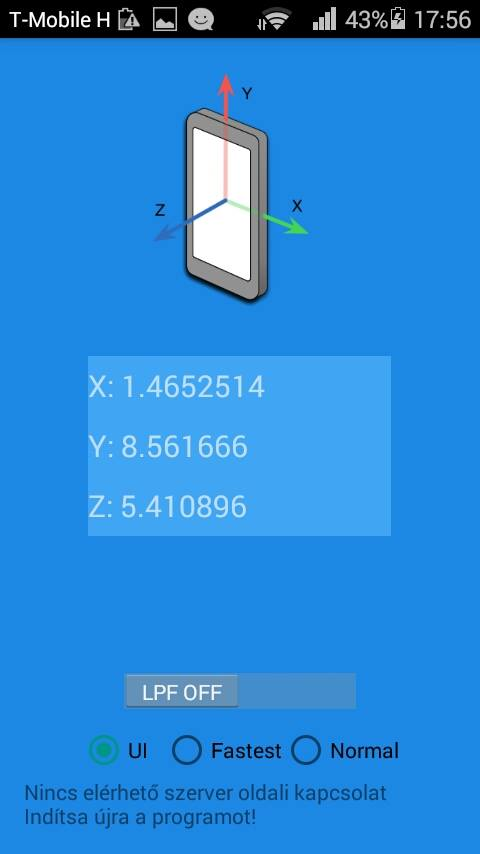
\includegraphics[width=6cm]{nincskapcsolat}
	\caption{Nincs elérhető kapcsolat}\label{nincskapcsolat}
\end{figure}

Ezt az Activity alján egy egyszerű Label-be írjuk ki, hogy figyelmeztessük a felhasználót. A kapcsolódás gombra kattintva (a kliens oldalon), az alkalmazás leellenőrzi hogy képes-e kapcsolódni, van-e olyan "elérési út", azaz IP cím amire kapcsolódni szeretnénk. Ezt a folyamatot a felhasználó nem látja, csak a későbbiek folyamán kap egy visszajelzést, hogy sikerült-e kapcsolódni vagy sem.
\par Abban az esetben, ha a szerver oldalon a kapcsolódást anélkül kíséreljük meg, hogy nincs elérhető internet kapcsolat, az alkalmazás erről is figyelmeztetést küld.
\par A kapcsolódást követően megkezdődik a kommunikáció. Ilyenkor a kliens elkezdi küldeni a szenzoradatokat a szerver felé. Ilyenkor már használhatóvá válnak a form-ra felhelyezett eszközök. Megkezdhetünk egy kísérletet. A kliens oldalon elérhető Switch segítségével az adatokat tudjuk megváltoztatni. Vannak esetek, amikor szükségünk van szűrésre, de vannak olyanok, amikor nem. Ez a lehetőség erre ad választási módot. Ezen felül szerepel még három RadioButton. Ezek arra hivatottak hogy a szenzor gyorsaságát tudjuk beállítani. Ez azért jó, mert ha például az ingáról beszélünk, fontos, hogy minél több adatot kapjunk meg, amiből dolgozni tud a szerver oldal. Minél kevesebb ez az adat, annál pontatlanabb eredményt kapunk.
\par A szerver oldalra visszatérve, a lehetőségeink tárháza elég nagy. A gyorsulás diagramon lehetőségünk van választani, hogy mely tengelyek gyorsulását szeretnénk látni. E mellett arra is van lehetőségünk, hogy a mobiltelefon aktuális pozícióját lementsük. Ez olyan kísérleteknél jöhet jól, ahol a kezdőállapottól függ a kísérlet végkimenetele.
\par A szenzoradatok mellett a klienstől érkezik egy negyedik adat is, ez pedig az idő. Az idő, olyan értelemben, hogy az első küldött adattól számítva mennyi idő telik el. Ez fontos lehet például abban az esetben ha sebességet, vagy hosszt szeretnénk kiszámítani.
\par Lehetőségünk van még továbbá arra is, hogy egy adott kísérlet során lementsük az adatokat. Ez a későbbi munkánkat tudja elősegíteni. Esetleg ha szeretnénk a későbbiekben felhasználni a kísérlet adatait, akkor ezek az adatok eltárolódnak egy TXT file-ba és a későbbiekben fel tudjuk azt használni.
\chapter{Összefoglalás}
Befejezésképpen összegzem a korábban leírtakat. Ehhez elevenítsük fel, az eredetileg megfogalmazott célokat.
\begin{quote}
	\it ,,...olyan Android alapú kliens applikáció, amely kapcsolatot tart egy szerveroldali alkalmazással. Ezeket a szenzoradatokat fizikai kísérletek mevalósítására, szemléltetésére használhatjuk fel, így a telefon egyfajta segédeszközzé válik."
\end{quote}
Ennek megfelelően a Visual Studio segítségével elkészítettem a szerveroldalt, amely tartja a kapcsolatot a mobil klienssel. Elégedett vagyok és sok tapasztalatot szereztem ezen fejlesztői környezet használatával, mivel könnyedén el tudtam készíteni a szenzoradat feldolgozó rendszert.
\par A szenzoradatok megértéséhez és azok megjelenítéséhez kutatnom kellett, és új dolgokat kellett megtanulnom, így az ismereteimet is bővíteni tudtam. Ez leginkább a diagram megjelenítésénél látszik igazán, hisz ott egy olyan beépített eszközt használtam, amivel azelőtt még nem volt dolgom.
\par Azon kívül, hogy a kész alkalmazás már használható arra a célra, amire ki lett találva, el kellett gondolkodnom a további fejlesztési lehetőségen is. Ez a téma, amit az első oldal óta boncolgattam számtalan irányból megközelíthető a továbbfejlesztést tekintve.
\par Az első és legfontosabb dolog, ami a bővítést említve eszembe jut, az a fizikai kísérletekre vonatkozik. A keretrendszer "rugalmasságának" köszönhetően ezen kísérletek megvalósítása csak a fantáziánkon múlik. Lényegében ha a telefont egy szimpla segédeszköznek tekintenénk, mint (a példa kedvéért) akár egy labdát, akkor kapcsolatot létesítve le tudnánk szűrni az adatokat, amelyek a kísérlet során történnek anélkül, hogy a látottak alapján megtippelnénk azokat.
\par Megközelíthetjük a fejlesztés ezen szakaszát szenzor oldalról is. Jelenleg az applikáció egyetlen szenzort használ, a gyorsulásmérőt. Mint már mondtam, ezt azért választottam, mert ez a szenzor található meg a telefonokban a leggyakrabban. Másrészt viszont, van még pár szenzor, amellyel más irányból is megközelíthetnénk ezeket a kísérletezéseket. Ilyen például a fényszenzor is. Tegyük fel, hogy valaki fénytani kísérleteket szeretne végrehajtani a telefon segítségével. Erre is van alkalmas szenzorunk, amellyel ezt akár meg is valósíthatjuk.
\par Végül de nem utolsó sorban megköszönöm a témavezető tanáromnak a bátorítást és a támogatást.Köszönöm mindenkinek, akik segítettek, ha kérdésem volt.

\begin{thebibliography}{1}
\bibitem{cimke} \textsc{Gyorsulásmérő}:\\\url{https://hu.wikipedia.org/wiki/Gyorsulás}
\bibitem{cimke} \textsc{Gyorsulásmérők a fizikában}\\ \url{http://www.mogi.bme.hu/TAMOP/mikromechanika/math-ch05.html#ch-V.2}
\bibitem{cimke} \textsc{Harmonikus rezgőmozgás}\\
\url{http://ecseri.puskas.hu/oktseged/mechanika/harmonikus_rezgomozgas.pdf}
\bibitem{cimke} \textsc{Szenzorok}\\
\url{http://users.nik.uni-obuda.hu/malk/android/ea_2011_tavasz/08_-_Szenzorok.pdf}
\bibitem{cimke} \textsc{AsyncTask}\\
\url{http://developer.android.com/reference/android/os/AsyncTask.html}
\end{thebibliography}
\end{document}
